%
% clip.tex
%
% (c) 2024 Lukas Schöpf, OST Ostschweizer Fachhochschule
%

% DeepL corrected
% explain Resnet and transformer

\chapter{Cross-modal networks
    \label{chapter:crossmodalnetworks}}
    Multimodal deep learning is the study of models that learn from multiple modalities. 
    For example, humans can use both vision and hearing to identify an object or a person. 
    Cross-modal deep learning leverages data from one modality to improve performance in another. 
    For instance, if a person looks at a picture of a bird and listens to its song, they might be able to identify the bird more effectively.

    One of its most impressive features is the ability to perform well on data the model has not been explicitly trained on. 
    This ability is known as zero-shot capability, which stems from N-shot capability. 
    N-shot capability refers to the number of training samples of a particular class that a model needs to classify it correctly.

    In this work, cross-modal networks are used to identify relationships between images and text. 
    Most cross-modal networks designed for this task consist of a text encoder and an image encoder.

    \section{Base Networks}
    To understand cross-modal networks, it is essential to first examine their components. 
    Most of these networks employ transformers as encoders, although some utilize ResNets. 
    The information presented in this section is derived from the corresponding paper and \cite{clipexplain}.

    \subsection{ResNet
    \label{crossmodalnetworks:sec:resnet}}

    Residual Networks (ResNets) were introduced in \cite{resnetpaper}. 
    A ResNet employs residual blocks (\cref{fig:crossmodalnetworks:resblock}), which incorporate residual connections between certain layers. 
    These connections allow information to bypass specific layers, facilitating the training of deeper networks by mitigating issues such as the vanishing gradient problem. 
    This mechanism stabilizes the training process and accelerates the convergence of deep neural networks. 
    The primary motivation for ResNets was to enhance image processing capabilities beyond those of traditional \acrfull{cnn}s. 
    Notably, large transformer models, such as OpenAI's GPT series, also utilize residual connections to improve performance and enable the training of deeper architectures \cite{attentionisallyouneed}.
    
    \begin{figure}[h]
        \centering
        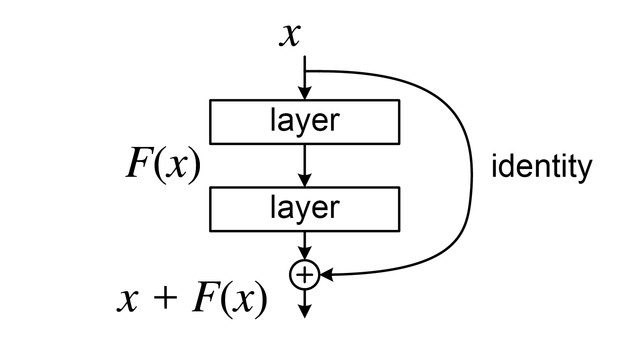
\includegraphics[width=0.55\textwidth]{Images/crossmodalnetworks/ResBlock.png}
        \caption{Image of a ResNet block.\cite{resnetpaper}}
        \label{fig:crossmodalnetworks:resblock}
    \end{figure}

    \subsection{Transformer}

    The Transformer was first introduced in \cite{attentionisallyouneed}.
    Most of the information in this section is derived from that paper. 
    Before Transformers, \acrfull{rnn}s were commonly used to process sequential data. 
    To capture dependencies and relationships within an input sequence, a mechanism called attention was introduced.
    The Transformer marked a significant breakthrough by introducing a mechanism known as self-attention.
    Self-attention does not need to be calculated sequentially.
    It is defined as:

    \begin{equation}
        \text{Attention}(Q, K, V) = \text{softmax}\left(\frac{QK^T}{\sqrt{d_k}}\right)V
        \label{equ:selfattention}
    \end{equation}

    where \(Q = XW_q\), \(K = XW_k\), and \(V = XW_v\). 
    Here, \(X\) represents the input, and \(W_{q}\), \(W_{k}\), and \(W_{v}\) are learnable parameter matrices. 
    The matrices \(Q\), \(K\), and \(V\) are referred to as query, key, and value, respectively. 
    The term \(\frac{1}{\sqrt{d_k}}\) is a scaling factor to normalize the output, where \(d_k\) is the dimensionality of the key vectors.
    
    Often, multiple attention heads are used simultaneously to allow the model to focus on different parts of the input sequence (see \cref{fig:crossmodalnetworks:attention}).
    
    \begin{figure}[]
        \centering
        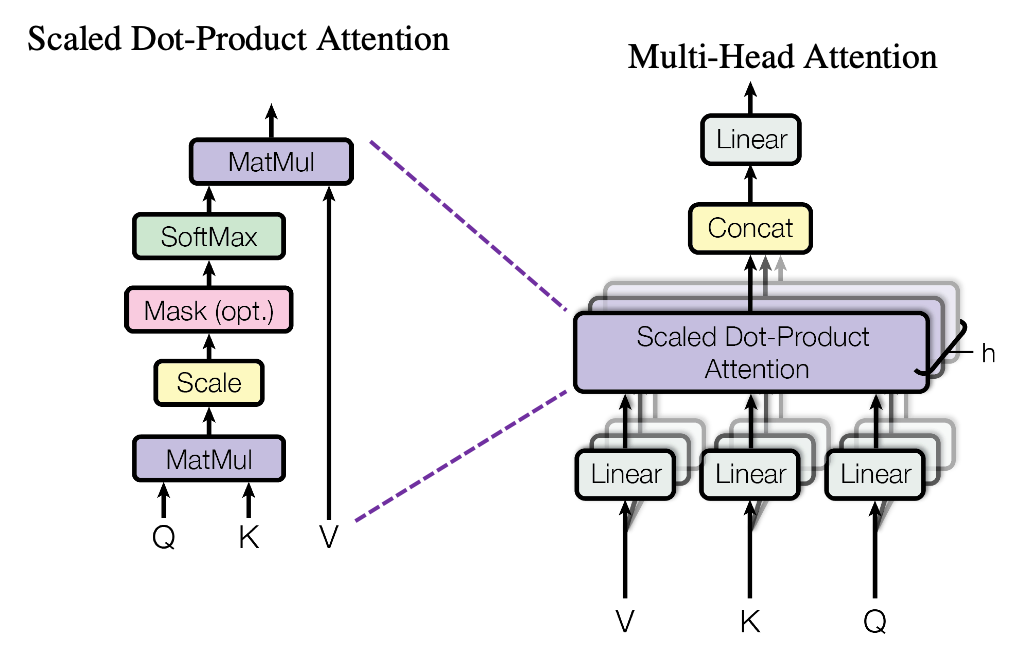
\includegraphics[width=0.7\textwidth]{Images/crossmodalnetworks/attention.png}
        \caption{Single and multi-head attention\cite{attentionisallyouneed}}
        \label{fig:crossmodalnetworks:attention}
    \end{figure}

    With the introduction of the self-attention mechanism, the need for \acrshort{rnn}s became obsolete. 
    \acrshort{rnn}s are challenging to train due to issues such as the vanishing or exploding gradient problem. 
    Additionally, they are difficult to parallelize because of their sequential nature. 
    These issues no longer occur when using a Transformer, as it processes sequences in parallel and effectively captures long-range dependencies.


    \begin{figure}[]
        \centering
        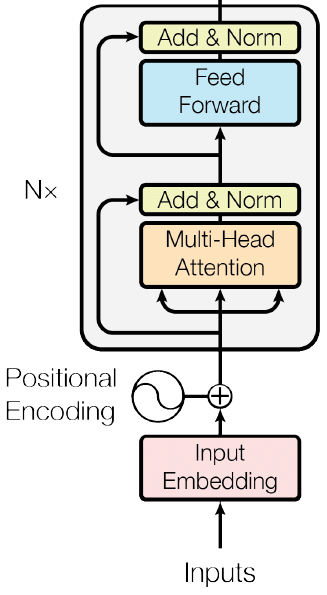
\includegraphics[width=0.25\textwidth]{Images/crossmodalnetworks/The-Transformer-encoder-structure.png}
        \caption{Image of a Transformer which in the case of CLIP is used as a text encoder\cite{attentionisallyouneed}}
        \label{fig:crossmodalnetworks:transformer}
    \end{figure}

    To use a Transformer, the input must first be split into tokens. 
    These tokens represent text snippets in the case of a text Transformer or patches of an image in the case of a Vision Transformer (ViT) (see \cref{fig:crossmodalnetworks:visiontransformer}). 
    These tokens or patches are then embedded into a high-dimensional vector space. 
    For example, in the case of the CLIP ViT-32 visual encoder, each vector has 1024 dimensions.

    Additionally, positional embeddings are added to the token embeddings to retain information about the order or spatial arrangement of the tokens. 
    Next, a combination of self-attention blocks and feed-forward layers is used to process the tokens (see \cref{fig:crossmodalnetworks:transformer}). 
    Residual connections and normalization are also employed to facilitate training.
    Multiple such blocks are concatenated to form the full Transformer architecture.

    \begin{figure}[]
        \centering
        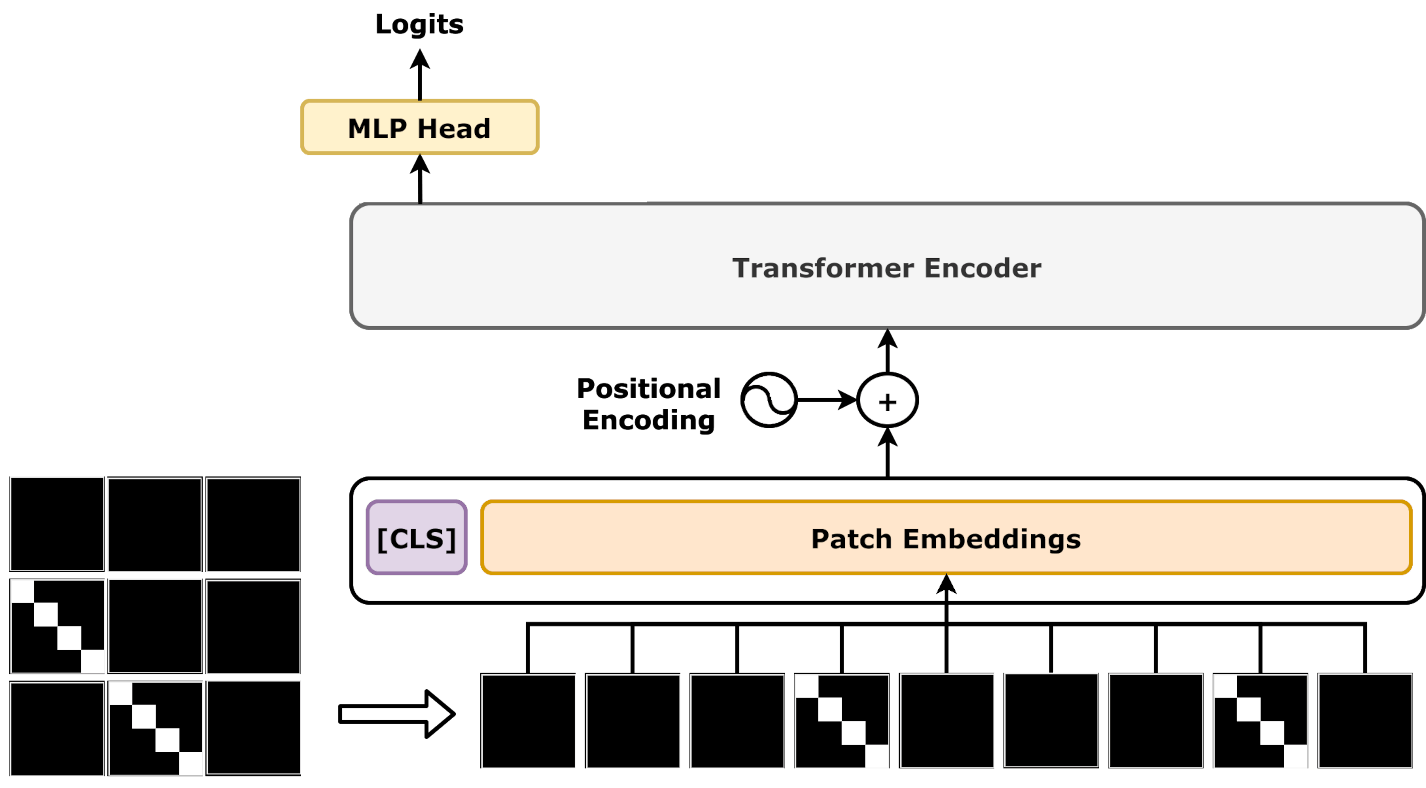
\includegraphics[width=0.6\textwidth]{Images/crossmodalnetworks/Vision_Transformer.png}
        \caption{Vision Transformer architecture\cite{vitwikipedia}}
        \label{fig:crossmodalnetworks:visiontransformer}
    \end{figure}

    \section{Text Encoder}

    The text encoder is typically implemented as a Transformer. 
    Its purpose is to encode a given text into a high-dimensional vector space. 
    This vector space enables the encoder to classify unseen classes by placing their vectors close to those of related classes. 
    In theory, the closer two words are related, the closer their corresponding embedding vectors are in the high-dimensional space.

    An example of this relationship can be visualized in \cref{fig:crossmodalnetworks:3demb}, where \acrfull{pca} is used to reduce the dimensionality of the embedding vectors. 
    For instance, the words "cat" and "dog" appear close together because they share a semantic relationship.

    \begin{figure}
        \centering
        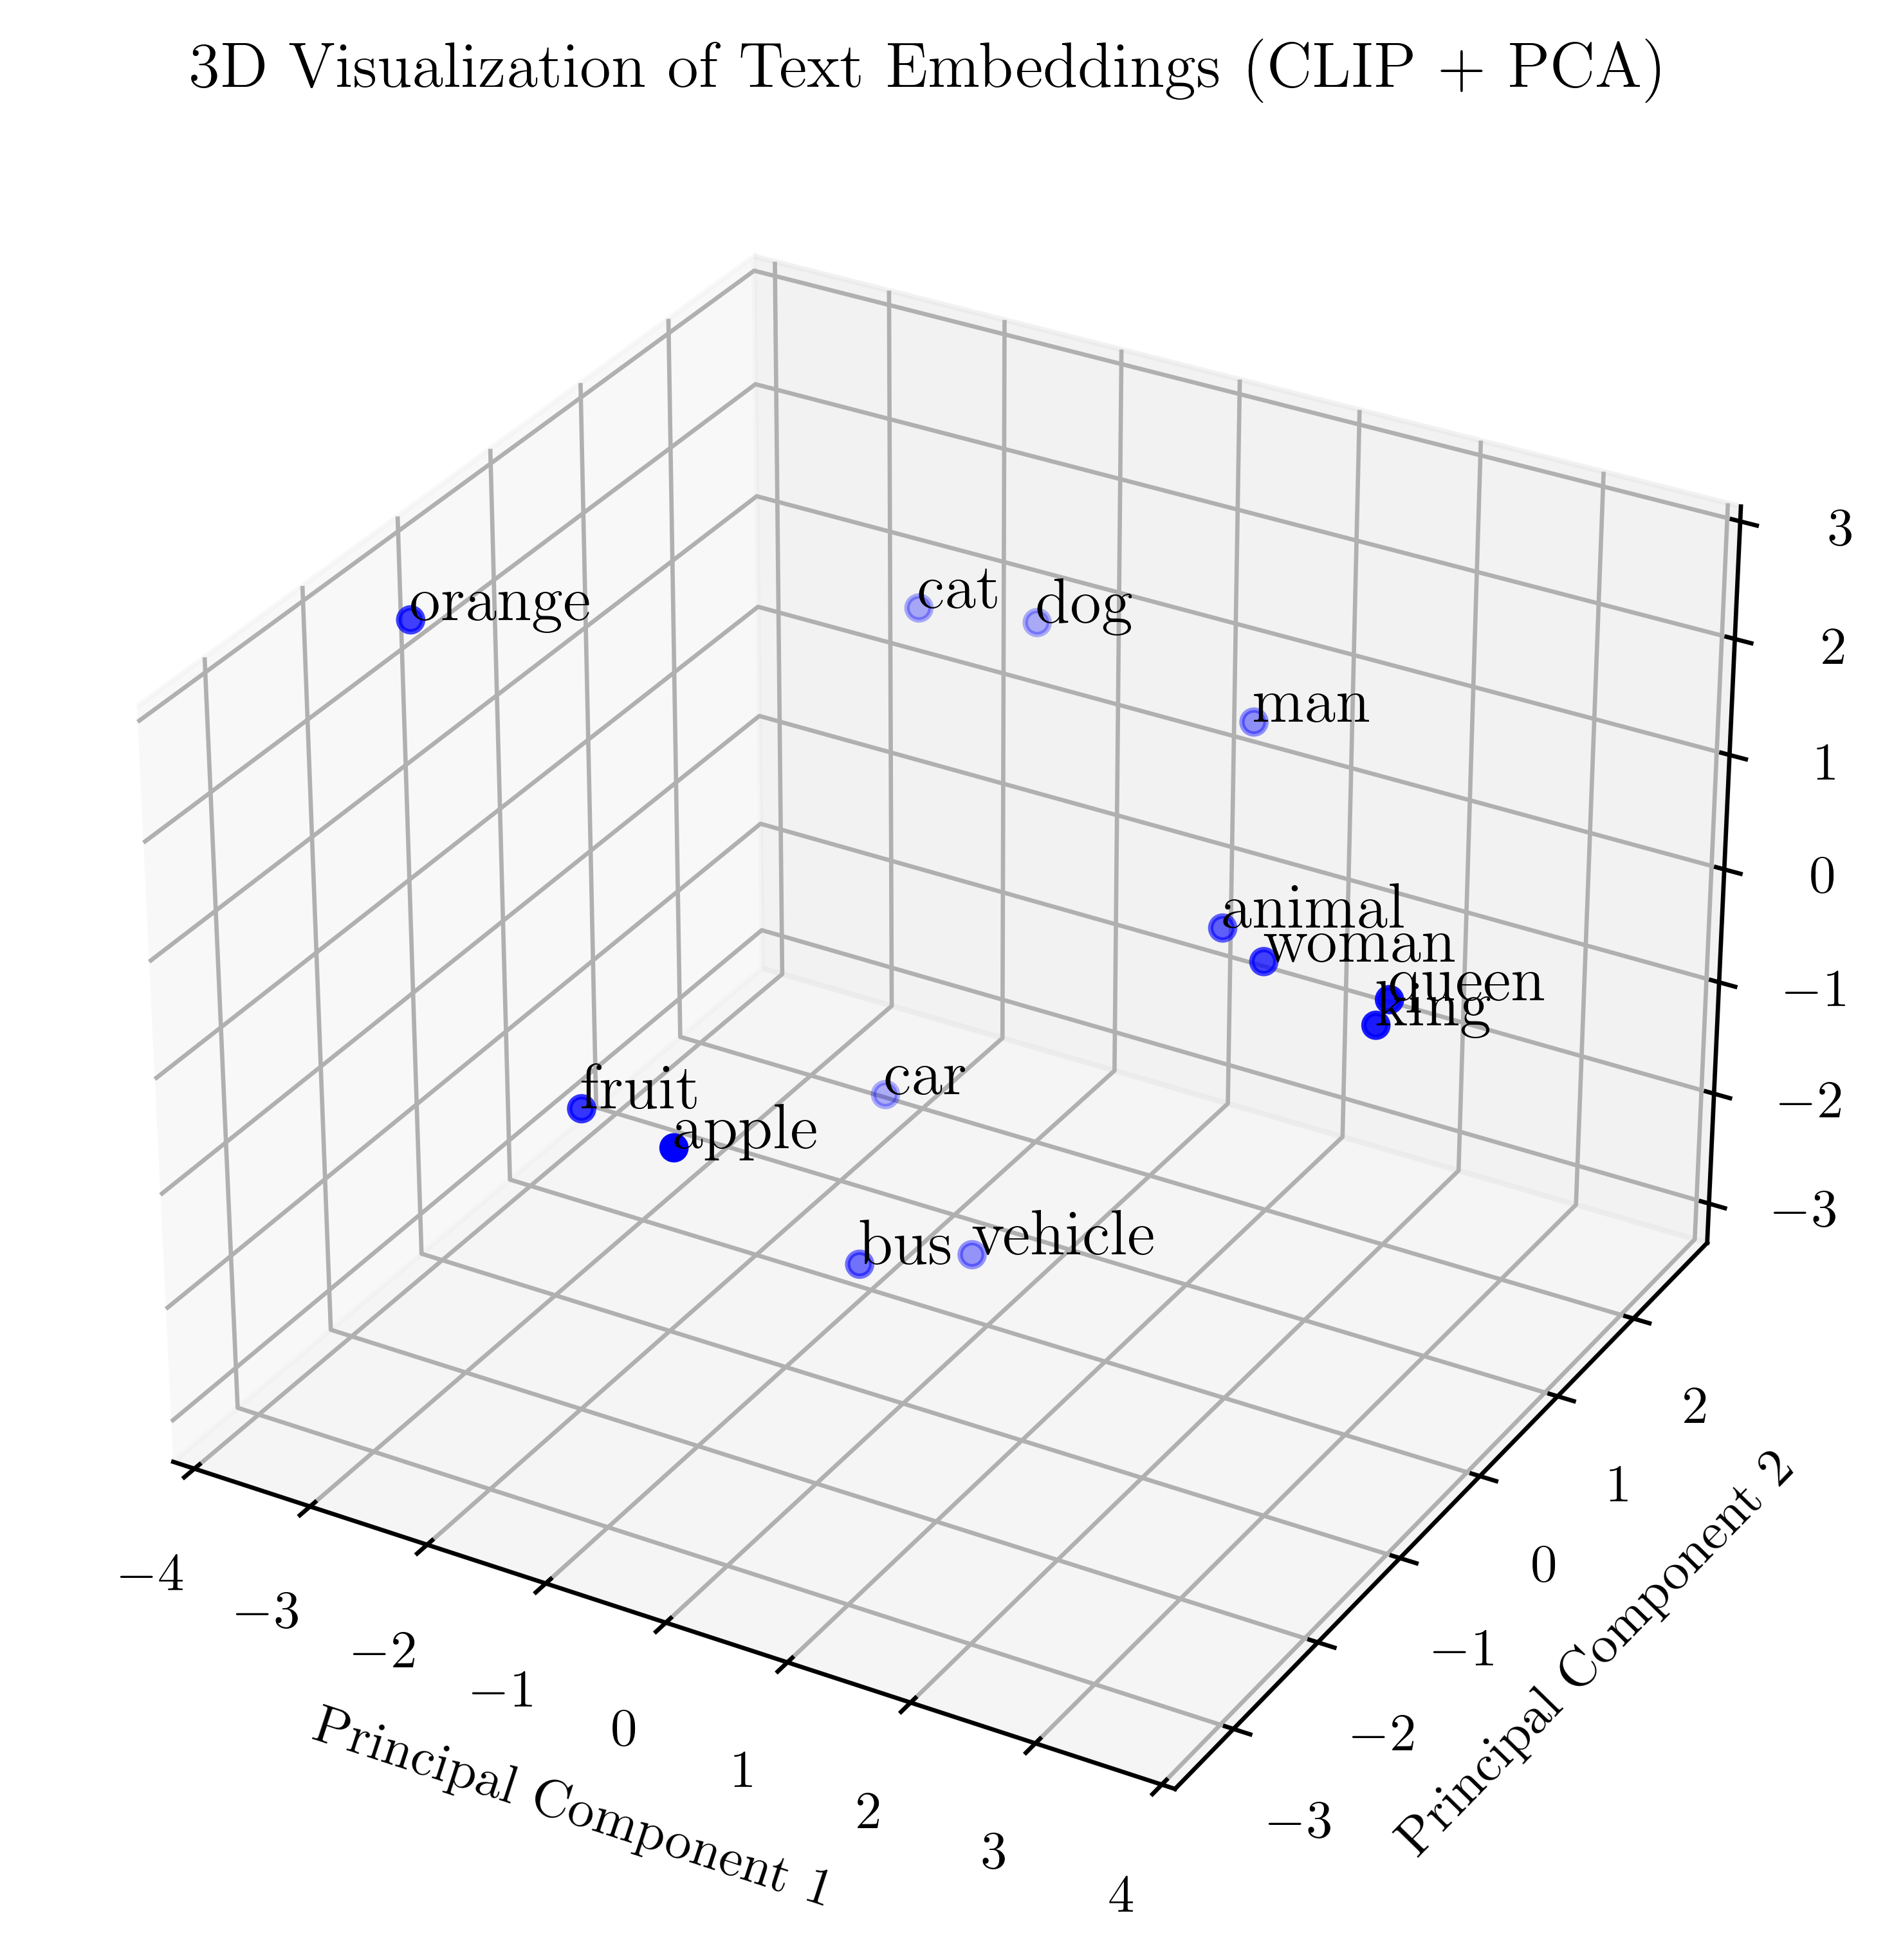
\includegraphics[width = 0.8\textwidth]{Images/crossmodalnetworks/3DEmbedding.png}
        \caption{Example of text embedding using CLIP and \Acrshort{pca}}
        \label{fig:crossmodalnetworks:3demb}
    \end{figure}
    
    \section{Image encoder}

    In most cases, the image encoder consists of a Vision Transformer \cite{Vis_N_Grams}. 
    Like the text encoder, the image encoder transforms an image into a high-dimensional vector space. 
    A Vision Transformer requires the input image to have a specific dimension. 
    For this reason, an image encoder typically consists of a Vision Transformer and a preprocessor, which transforms the image into the correct dimensions for the Vision Transformer.

    \section{Contrastive Language-Image models
        \label{section:languageimagemodels}}
        This section explores models that use both text and image modalities. 
        Most of the information in this section is derived from \cite{cliplikeweb} and related papers.

        Contrastive techniques involve paired inputs from two modalities (e.g., an image and its corresponding caption). 
        Each input is embedded into its own embedding space. 
        The goal is for such pairs to be represented in similar embeddings by their respective encoders. 
        The term "language-image" refers to the two modalities used by the model. 
        Most of these models are pre-trained on large, general datasets. 
        Pre-training means that the model has been trained on a broad, universal dataset. 
        For a specific application, a pre-trained model can be fine-tuned to improve its performance on the targeted task.

        \subsection{CLIP
            \label{section:clip}}
        \acrfull{clip} \cite{clip} is a cross-modal model developed by OpenAI \cite{openai} that evaluates how well a given image and text match. 
        It can be used with various image and text encoders. 
        The model is trained on a large dataset consisting of 400 million image-text pairs. 
        \acrshort{clip} has been shown to outperform some of the best-known models in image classification. 
        Many other models build upon \acrshort{clip} as a foundation, improving upon it to create more advanced architectures.
            

        \begin{figure}[]
            \centering
            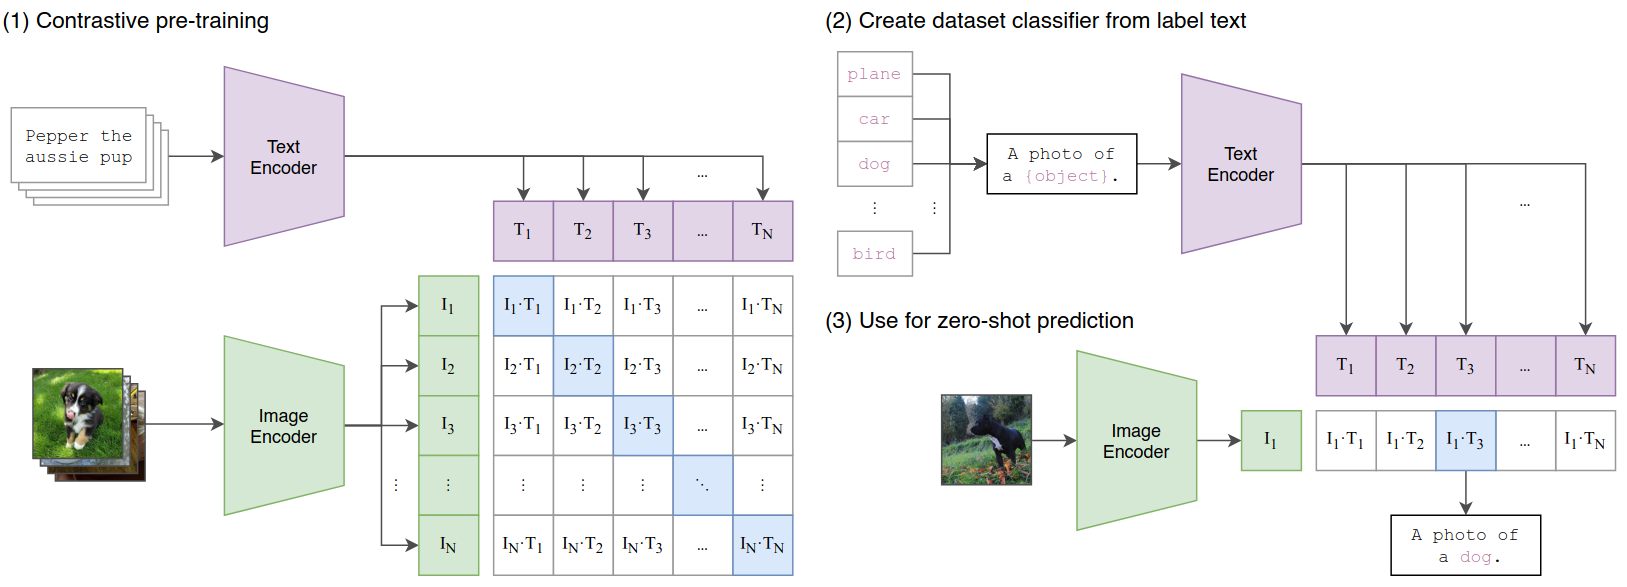
\includegraphics[width=\textwidth]{Images/crossmodalnetworks/OpenAICLIP.png}
            \caption{A picture from the \acrshort{clip} paper by OpenAI \cite{clip}.}
            \label{fig:crossmodalnetworks:openaiclip}
        \end{figure}

        \subsection{ALIGN
            \label{section:align}}
        \acrfull{align} \cite{ALIGN} was released shortly after \acrshort{clip}. 
        Rather than relying on small image-caption datasets, \acrshort{align} uses a dataset of 1.8 billion image-alt-text pairs (e.g., as shown in \cref{fig:crossmodalnetworks:alignepairs}). 
        These alt-text descriptions are much noisier than captions. 
        The authors apply basic filtering techniques to remove duplicates, images with more than 1000 associated alt-texts, and uninformative alt-texts (such as those that are either too frequent or contain rare tokens), while avoiding expensive filtering operations. 
        With these simple steps, \acrshort{align} meets or exceeds the state-of-the-art performance on several zero-shot and fine-tuning tasks.
            
        \begin{figure}
            \centering
            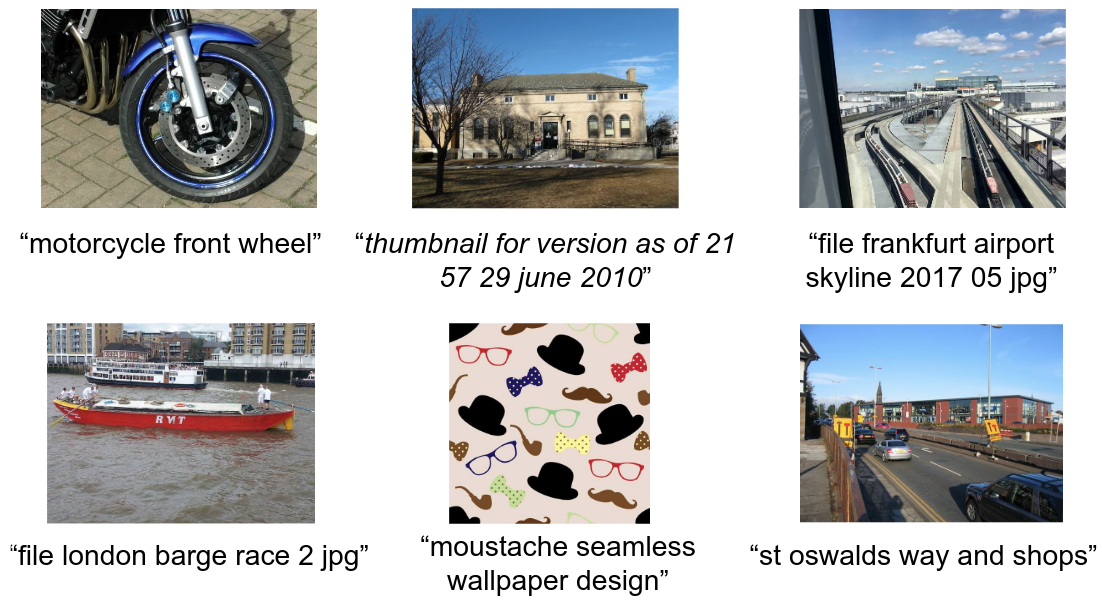
\includegraphics[width=\textwidth]{Images/crossmodalnetworks/examplepicsalign.png}
            \caption{Example of alt-text image pairs from the train dataset from \acrshort{align}\cite{ALIGN}}
            \label{fig:crossmodalnetworks:alignepairs}
        \end{figure}

        In a test described in this paper, \acrshort{align} was much slower than \acrshort{clip} when performing a zero-shot evaluation on the CIFAR100 \cite{cifar100} dataset. 
        For a single prediction, \acrshort{align} takes 70 times longer than \acrshort{clip} (see \cref{tab:clipaligntest}). 
        Neither of the networks were fine-tuned, and the highest predicted label was used. 
        Due to the slow inference speed, ALIGN was stopped after processing 35\% of the dataset.

        \begin{table}
            \centering
            \begin{tabular}{lll}
                \hline
            \textbf{Measurment}&\textbf{ALIGN}&\textbf{CLIP}\\\hline
            Accuracy& 48.9\% & 61.7\%\\
            Speed(seconds per iterarion)&  2.16&  0.02\\ \hline
            \end{tabular}
            \caption{First test on CIFAR100.}
            \label{tab:clipaligntest}
        \end{table}

        \subsection{TinyCLIP
            \label{section:tinyclip}}
        \begin{figure}
            \centering
            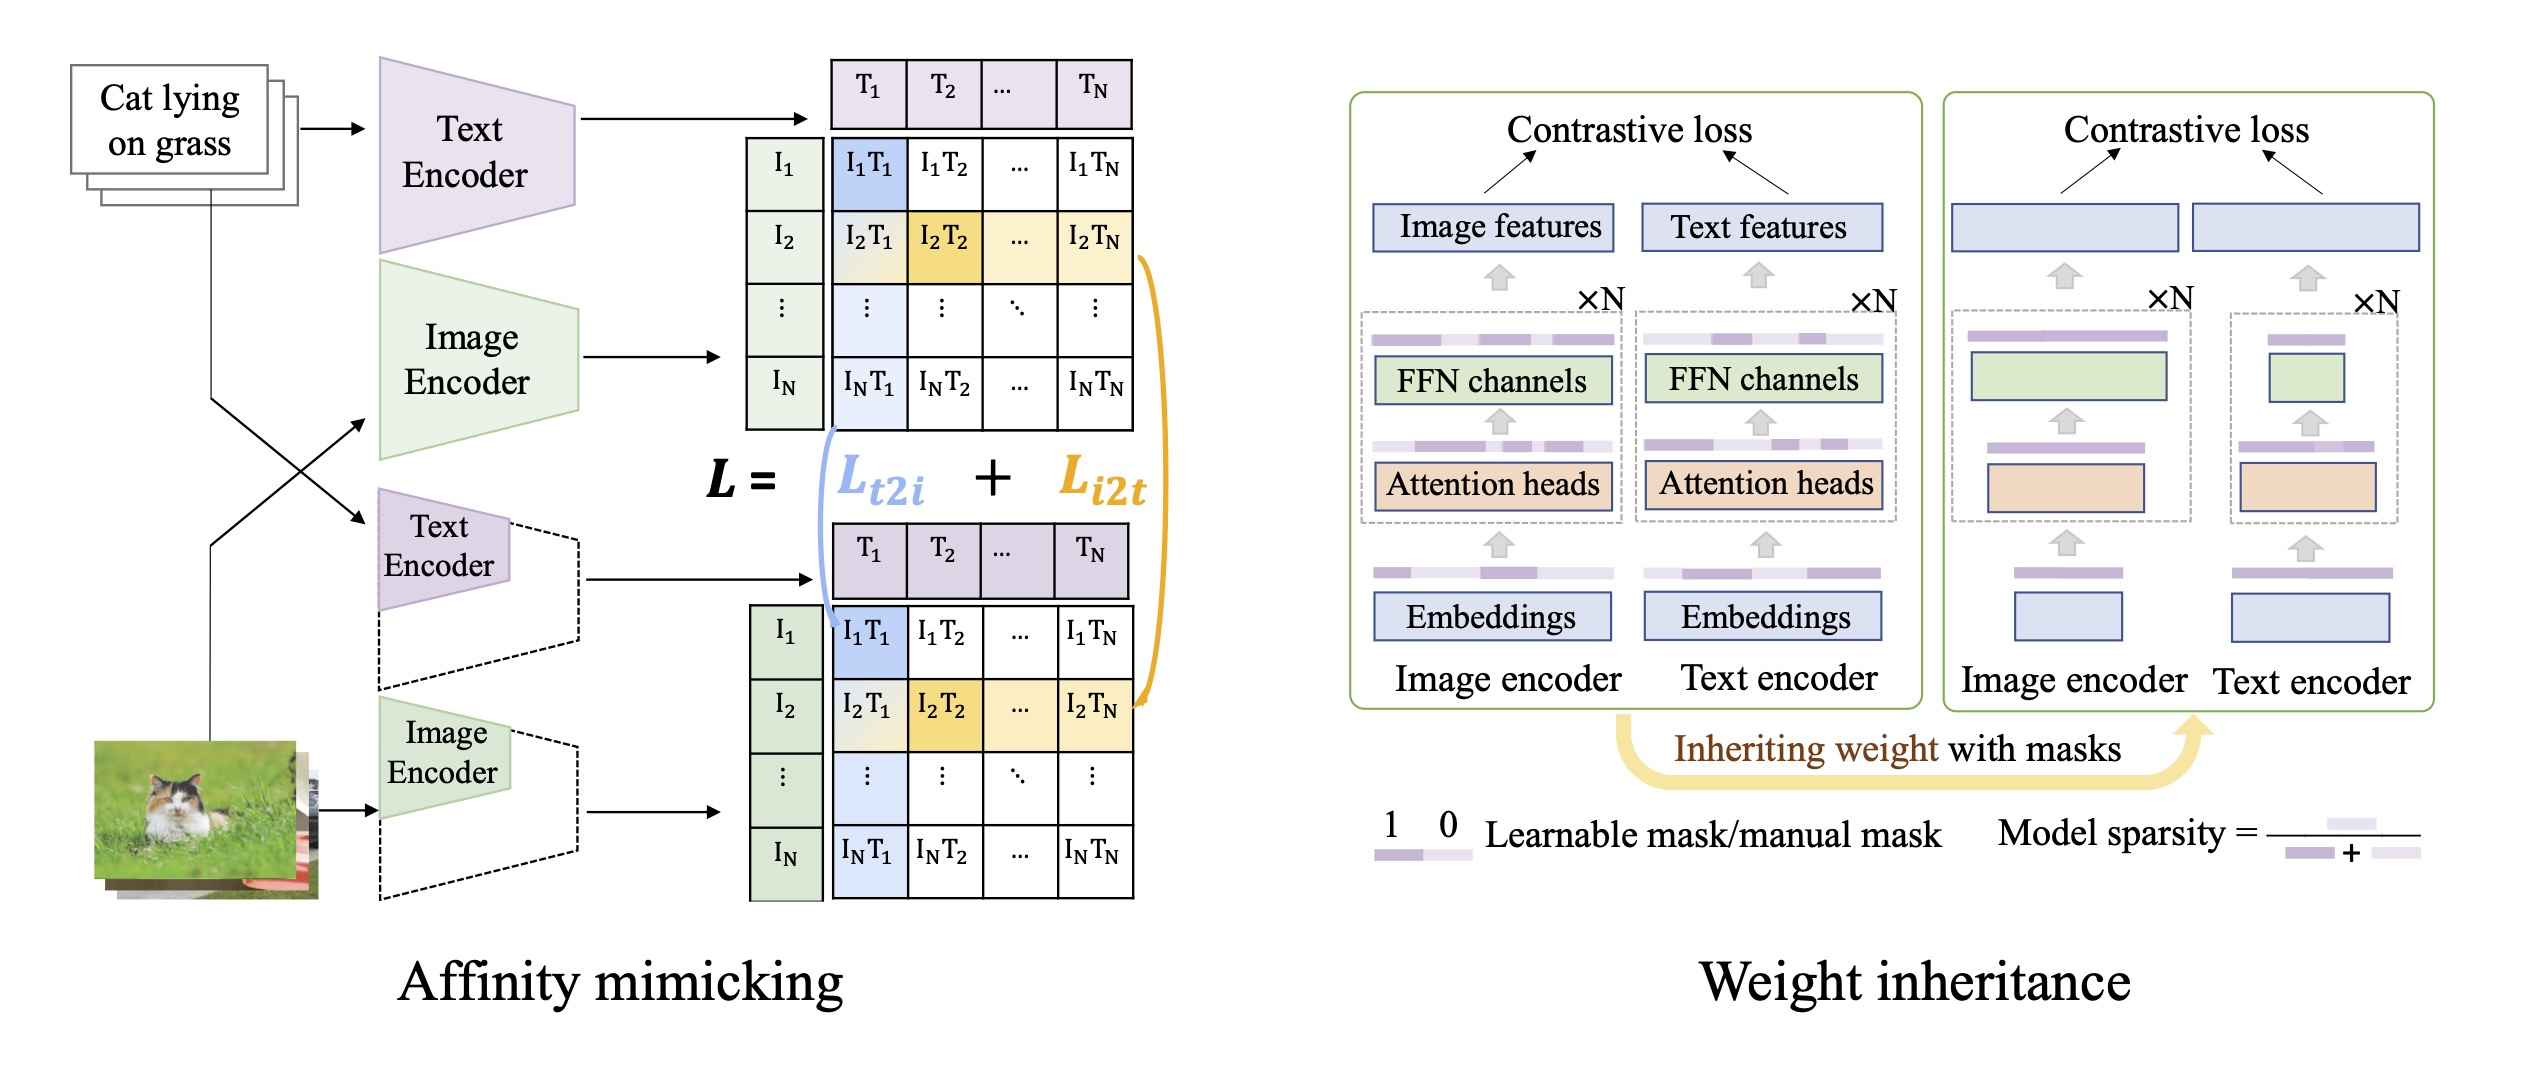
\includegraphics[width=\textwidth]{Images/crossmodalnetworks/TinyCLIP.jpg}
            \caption{Optimization which are used in TinyCLIP\cite{tinyclip}}
            \label{fig:crossmodalnetworks:tinyclip}
        \end{figure}

        TinyCLIP \cite{tinyclip} is a cross-modal distillation method designed for large-scale pre-trained speech-image models. 
        TinyCLIP can be used on resource-limited systems due to its miniaturization. 
        It also accelerates training with minimal loss in model accuracy. 
        The method utilizes three key concepts to reduce the size of the network.


        \subsubsection{Affinity mimicking}
        Affinity mimicking is a specialized form of knowledge distillation, also known as model distillation. 
        In knowledge distillation, a larger teacher network is trained first. 
        After training the teacher network, a smaller student network is trained to predict the output of the teacher network. 
        This approach works because the output of the teacher network contains more information than the original label. 
        Affinity mimicking introduces two new metrics in the training process: language-to-image loss and image-to-language loss (\(L_{t2i}\) and \(L_{i2t}\), as shown in \cref{fig:crossmodalnetworks:tinyclip}).


        \subsubsection{Weight inhertiance
        \label{section:weightinheritance}}
        Weight inheritance is a technique that transfers important weights from well-trained teacher models to smaller student models. 
        In the paper, the authors propose two methods:
        \begin{itemize}
            \item \textbf{Manual weight inhertiance:} Based on the authors' observations, text encoders exhibit the most redundancy in depth (layer-wise), while image encoders exhibit redundancy in width (channel-wise). 
            They select \(k\) layers and channels from a branch to serve as initialization weights. 
            To select the most important weights, some prior knowledge is required.
            \item \textbf{Automatic weight inhertiance:} The authors introduce a learnable mask to determine the importance of each weight.
        \end{itemize}

        \subsubsection{Multi-stage progressiv distillaiton}
        The model is pruned in several steps. 
        At each stage, the authors apply a modest degree of compression (e.g., 25\%). Each stage also includes weight inheritance and affinity mimicking.
        

\section{Enhance the algorithm
    \label{section:enhancealgorithm}}

    To improve the accuracy of a pre-trained network, it can be fine-tuned for a specific task. 
    Fine-tuning is a broad term, encompassing methods ranging from the simple addition of a learnable linear layer at the end of the network to feature distillation. 
    The concept of fine-tuning is derived from transfer learning \cite{transferlearning}, where the final layers of a neural network are removed and the network is retrained with new, independent layers. 
    This approach saves time and resources. 
    For example, in CLIP, a linear layer can be added to enhance classification performance \cite{finetuneclip}. 
    All fine-tuning approaches rely on the output of the network for further processing. 
    Another way to increase accuracy is by using better-fitting text prompts.
    
\section{Conclusion multi-modal networks}
    Based on the results of our own testing, ALIGN is not considered a suitable solution for this work. 
    Instead, the focus is on CLIP and TinyCLIP, which can be fine-tuned to further improve their performance. 
    Additionally, the performance of these models can be enhanced by using more effective text prompts.